\documentclass{article}
%\usepackage{nips_2016}
\usepackage[maxfloats=250]{morefloats}
% to compile a camera-ready version, add the [final] option, e.g.:
\usepackage[final]{nips_2016}
% \usepackage{morefloats}
\usepackage[utf8]{inputenc} % allow utf-8 input
\usepackage[T1]{fontenc}    % use 8-bit T1 fonts
\usepackage{hyperref}       % hyperlinks
\usepackage{url}            % simple URL typesetting
\usepackage{booktabs}       % professional-quality tables
\usepackage{amsfonts}       % blackboard math symbols
\usepackage{nicefrac}       % compact symbols for 1/2, etc.
\usepackage{microtype}      % microtypography
\usepackage{graphicx}


\title{Wasserstein-InfoGAN for the Identification of Targeted Linear Basis Expansions and Applications to Classical Methods of Dimensionality Reduction and Inverse Problems  }

\author{
  Charlie Talbot\thanks{Use footnote for providing further
    information about author (webpage, alternative
    address)---\emph{not} for acknowledging funding agencies.} \\
  Department of Mathematics\\
  University of North Carolina at Chapel Hill\\
  Chapel Hill, NC 27514 \\
  \texttt{hippo@cs.cranberry-lemon.edu} \\
  %% examples of more authors
  %% \And
  %% Coauthor \\
  %% Affiliation \\
  %% Address \\
  %% \texttt{email} \\
  %% \AND
  %% Coauthor \\
  %% Affiliation \\
  %% Address \\
  %% \texttt{email} \\
  %% \And
  %% Coauthor \\
  %% Affiliation \\
  %% Address \\
  %% \texttt{email} \\
  %% \And
  %% Coauthor \\
  %% Affiliation \\
  %% Address \\
  %% \texttt{email} \\
}
\begin{document}
\maketitle

\begin{abstract}
Methods of machine learning are being applied with increasing frequency to problems in science and engineering.  In many fields, however, applications are limited by the quantity of quality data.  This is especially true in the context of geophysics, where classic methods of dimensionality reduction have been been applied to the solution of inverse problems.  It has been shown, though, that PCA and its nonlinear extension applied to small quantities of highly heterogeneous dataare unlikely to facilitate optimization  The increasing interest in and extensions of Generative Adversarially Networks (GAN) has led to developments which have increased the stability of training generative networks resulting in realistic natural images.  We apply these to the task of generating realizations of geophysical media that can be used as an alternative surrogate to popular methods such as the Single Normal Equation Simulation (SNESIM) algorithm.  In particular, we combine ideas from (Kernel) PCA and GAN, combined with a convolutional neural networks, variational extensions presented in InfoGAN and minimization via the Wasserstein metric to create a stable algorithm for generating surrogate channelized media.  We present this generative model as an improvement to methods used previously to generate surrogate media, and discuss its utility in a recent method devised for the solution of inverse problems using dimensionality reduction techniques.  Finally, we present an extension using PCA (or a general autoencoder) in a way that bypasses the complexity of inverting the GAN to determine a decomposition of a given image in terms of its latent variables.
\end{abstract}

% PPCA \cite{Tipping1999ProbabilisticAnalysis}
% KPCA \cite{Scholkopf1997KernelAnalysis}
% MXKPCA \cite{Ma2011KernelGeneration}
% Oberai \cite{Oberai2003SolutionMethod}
% GAN \cite{Goodfellow2014GenerativeNetworks}
% DCGAN \cite{Radford2015UnsupervisedNetworks}
% WGAN \cite{Arjovsky2017WassersteinGAN}
% infoGAN \cite{Chen2016InfoGAN:Nets}
% EBGAN \cite{Zhao2016Energy-basedNetwork}
% BEGAN \cite{Berthelot2017BEGAN:Networks}
% ALI \cite{Dumoulin2016AdversariallyInference}

\section{Introduction}
The application of methods of machine learning to the formation of stochastic input models and the solution of inverse problems has been of increasing interest in recent years.  These methods are, however, limited by the quantity of high quality data, often in the context of geophysics, especially in the topology of the subsurface.  The increasing interest in and extensions of Generative Adversarial Networks (GAN) has led to developments which have increased the stability of training generative networks to produce realistic natural images.  We apply these to the task of generating realizations of geophysical media that can be used as an alternative surrogate to computationally expensive methods such as the Single Normal Equation Simulation (SNESIM) algorithm.  In particular, we combine ideas from (Kernel) PCA and GAN, combined with  convolutional neural networks, variational extensions presented in InfoGAN and minimization via the Wasserstein metric to create a stable algorithm for generating surrogate channelized media.  We present this generative model as an improvement to methods used previously to generate surrogate media, and discuss its utility in a recent method devised for the solution of inverse problems using the adjoint method combined with dimensionality reduction techniques.  Finally, we apply an extension using PCA (or a general autoencoder) in a way that bypasses the complexity of inverting the GAN to determine a decomposition of a given image in terms of its latent variables (GAN codes).

\begin{figure}[h]
\centering
  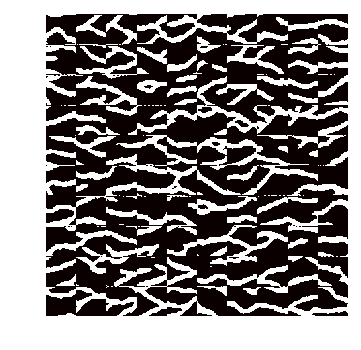
\includegraphics{figures/OptSnapshots_32.png}
  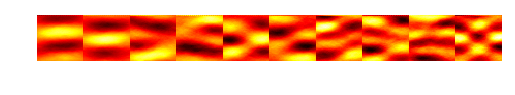
\includegraphics{figures/OptSnapshots_32_Modes.png}
  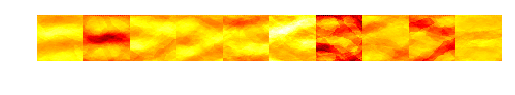
\includegraphics{figures/OptSnapshots_32_Modes_KPCA.png}
  \caption{(top) $100$ realizations of a channelized medium, linear (middle) and kernel principal modes }
\end{figure}\label{Snapshots}

\subsection{Background}

\subsection{Generative Adversarial Networks and Recent Extensions}
	The Generative Adversarial Network, the brainchild of Goodfellow et al in \cite{Goodfellow2014GenerativeNetworks} marked a departure from traditional neural network architectures in that it consisted of an objective inspired by game theory in which two neural networks are engaged in a zero-sum game.  The interplay of the two networks separate purposes--a generator, with the objective of producing realistic images from samples of common univariate distributions and a  discriminator with the opposing aim of distinguishing real and generated data--naturally leads to a min-max objective.  While highly effective at generating surrogate data that is similar and representative of the structure o the input data, the optimization objective of the original GAN proved highly nonconvex, leading to unstable and unreliable training with common modes of failure.  Notorious among these failure modes is the 'collapse' of the generated images to a single output.

	The potential of GANs for generation of natural images led to extensions using deep convolutional networks to produce a model that effectively captured a sort of linear algebra of features within images.  Further improvements upon the method continue to be made, though in many ways the instability of the GAN seems to have been improved significantly by a re-interpretation the minimax objective as being related to underlying distributions of real and generated data \cite{Arjovsky2017WassersteinGAN}. Not only does this re-formulation of the objective lead to training with increased stability and decreased occurence of common failure modes, but also leads to a more readily interpretable objective that can be used as a convergence criterion. Other methods, such as that derived in \cite{Chen2016InfoGAN:Nets}, yield latent variable representations of the data through methods of unsupervised learning.  Such a model has untapped potential in its applications to physically-inspired problems.

\subsection{Applications of Dimensionality Reduction to Geophysical Problems }\label{intokpca}
	A common problem in the context of geophysics/geodynamics is to recover the topology and geoemetry of a medium given a noisy measurement of deformation.  Such problems include seismic waveform inversion and determination of preferred flow pathways in channelized media.  At present we are concerned with the latter: given a deformation of a channelized medium, we wish to reconstruct the domain.  Consider the examples of Figure \label{Snapshots}; these 100 instantiations of a channelized medium respect certain, unknown multipoint statistics, and are unlabeled. We seek to use a modified GAN to categorize complex features and generate realistic snapshots that can be continuously mapped to nearest neighbors according to some unknown similarity metric.  Modes from PCA (Middle) and  the pre-image of the high dimensional image of mapping defined by KPCA (Bottom) show that the basis captures either limited, linear structure in the data (PCA) or of modes representing mixtures of realizations of the original data.
    
    Determining the medium, given a measurement of deformation, entails solving an inverse problem. In the event where the deformation (a 2-Dimensional image) is of high dimensionality relative to the number of samples, a common technique for determining the structure of the domain, given the output deformation, is the adjoint method.  
	In brief, the adjoint method can be thought of as follows: given a model with a known input and a high-dimensional target, one can engage in an efficient optimization procedure by re-associating terms in the model carefully to determine gradients with respect to a lower dimensional product, thereby decreasing the number of variables one must optimize with respect to \cite{Oberai2003SolutionMethod}.  Such a gradient is known as the adjoint gradient.
Extensions to the method have been recently been devised using Kernel PCA.  This was inspired by the use of the technique for generation of realizations for stochastic input models of fluid flow \cite{Ma2011KernelGeneration}.  Realizations (images, snapshots) of a channelized medium are generated from a Single Normal Equation Simulation (SNESIM) algorithm using multipoint statistics of a training image ($250 \times 250$ pixel) proposed to represent structure and properties (Young's Modulus) of the medium.  Linear or Kernel PCA are used on these training realizations to determine a basis which, through automatic differentiation, can be used with the adjoint gradient to optimize with respect to a reduced set of coefficients in the Principal Component Basis.  While the method has shown some success on training data, its effectiveness is limited to test data (unknown, target input images of channelized media generating the given deformation) bearing close resemblance to training images.
	To enhance the effectiveness of the method, the present author derived a sample-Weighted extension to Kernel PCA (WKPCA).  Still, due to the limited generative powers of PCA (discussed further in \label{related}) and limited quantities of data (both input channelized media and deformations) the problem remains unresolved.  For example, consider Figure \label{KDEPCA}.  Cumulative explained variance (not shown) for a truncated discrete Karhunen-Loeve expansion, PCA (top), indicates that $100$ of the $1000$ modes in total for the small channelized media dataset explain 90 percent of the variance in the data.  We use cross-validation to determine the bandwidth of the Kernel Density Estimator  Sampling random variable coefficients in the PC basis generates data that is structurally the same as the original data, as is expected from linear methods.  For the same procedure applied to Kernel PCA with a third degree polynomial kernel (bottom) the nonlinearity introduced by KPCA fails to do better, likely the result of the associated difficulties with pre-images of mappings induced by kernel methods.

	Creating modified GAN with the key improvements mentioned, we aim to generate meaningful representations of channelized media from small amounts of data.  We show how a deep convolutional GAN incorporating the Wasserstein metric and maximization of mututal information between a set of latent variables and the available data can furnish a powerful representation of the medium.  We further discuss the capability of the method to provide a means of determining weights for WKPCA for use the solution of inverse problems using the Adjoint Method.

\begin{figure}[t!]
  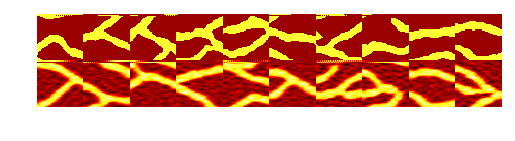
\includegraphics[width=\linewidth,scale=0.1]{figures/OptSnapshots_32_KDESamples100.png}
  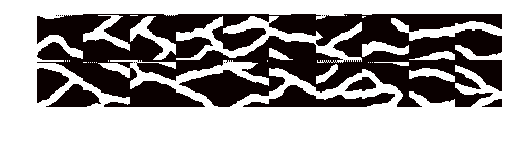
\includegraphics[width=\linewidth,scale=0.1]{figures/OptSnapshots_32_KDESamples100_KPCA.png}
  \caption{A simple generative model using KDE in the Linear (Top) and Kernel (Bottom) principal component bases. }
\end{figure}\label{KDEPCA}

% \cleardoublepage

\begin{figure}[h]
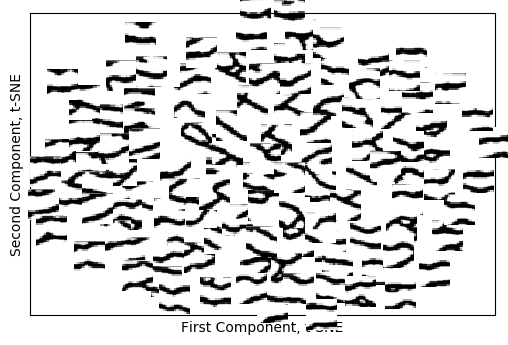
\includegraphics[width=\linewidth,scale=0.05]{figures/OptSnapshots_32_tSNE2.png}
  \caption{t-SNE applied to the data constituting realizations of a channelized medium.  Both 2D and 3D (not shown) embeddings of the data reveal that standard dimensionality reduction techniques do not yield any apparent grouping or clustering of the data.  This prevents meaningful segregation of data so as to attribute significance weights in WKPCA. }
\end{figure}\label{tSNE}

\section{Related Methods}\label{related}
% \subsection{DC-GAN}
	We review the methods on which our neural network architecture is based following a discussion the limitations of previous methods applied to the inverse problem for the images of the channelized media considered.
\newline
\subsection{Limitations of the use of Kernel PCA with Adjoint-Based Optimization }\label{limkpca}
	As discussed previously in \label{intokpca}, attempts were made using Linear or Kernel PCA applied to a small dataset in the hope that this will yield an optimal basis with respect to which one may optimize so as to solve an inverse problem.  This, as shown in \label{KDEPCA}, encounters at least two issues.  First and most evident is that, while the normally distributed coefficients in the principal component basis (or those distributed otherwise in the basis of kernel PCA for a given kernel) can be used to generate distinct realizations of the data, these generations are structurally/qualitatively the same, as they are constrained by linear combinations of basis vectors in the case of PCA.  While Kernel PCA may appear to offer some hope of addressing by nonlinearity.  However, KPCA is essentially carrying out the singular value decomposition in a higher dimensional space, and it is possible (if not likely) that the pre-image to realizations generated by KPCA may not exist or, if it does, may not be unique \cite{Scholkopf1997KernelAnalysis}.  By the very nature of PCA, one might expect that vectors in the basis corresponding to, for example, the MNIST data may not be individually representative of digits, but rather mixtures that maximize the variance of that mode.  From another perspective: many datasets are comprised of realizations that do not necessarily correspond to data that is labeled or naturally belong to some immutable category. As the basis (principal modes) determined by PCA is sensitive to outliers, the modes resulting from singular value decomposition applied to data with significant variations will again maximize the variance of components of the transformed data by forming linear combinations of data that one would hope to distinguish. Hence we need a more powerful, nonlinear model that is, by contrast, generative in nature. 


\subsection{InfoGAN}\label{igan}
	The original GAN architecture creates a generative model in terms of a reduced set of codes expressed in terms of random variables.  But, it is well-known that the values of these codes do not necessarily have any direct relationship with the output generated, leading to representations that are in some sense entangled.  To address this, the authors in \cite{Chen2016InfoGAN:Nets} devise InfoGAN, an information-theoretic extension to the original GAN architecture is devised to yield a meaningful representation of data in terms of a reduced set of variables $c$ in an unsupervised manner by aiming to maximize mutual information $I(c;G(z,c))$ between a set of latent variables and subsets of the data.  As derived in \cite{Chen2016InfoGAN:Nets}, the auxiliary distribution (associated with the auxiliary /variational/Q-network) in the variational upper bound for approximating the conditional distribution of a latent variable given a data sample. This is shown by the authors to be such that, as the auxiliary distribution approaches the true posterior distribution, the KL-Divergence from $P(c|x)$ (where $c$ denotes a latent variable) to $Q(c|x)$ vanishes. As this occurs, the variational upper bound becomes tight, as it is bounded below by the entropy of the latent codes $H(c)$.
\newline
	The authors demonstrate that this procedure results in codes that classify digits in an unsupervised manner, detect the absence or presence of more complicated features such as pose, lighting, and orientation.  The model of % infoGAN \cite{Chen2016InfoGAN:Nets}
 is furthermore attractive not only due to its ability to in essence detect and segment categorical and continuous changes in data, but to do so efficiently, adding only a minimal cost by using outputs of the discriminator.  Since we are interested in both generating new data and understanding its relationship to existing data so as to determine continuous transformations of a given image not represented in the original dataset, we incorporate the minimization of mutual information of InfoGAN in our model. 


\subsection{Wasserstein GAN }\label{wgan}
%WGAN
	As noted by a variety of authors, the (originally, Mini-Max) optimization objective of GAN is both significantly different from traditional objectives used in neural networks and is simultaneously highly nonconvex.   As described in the example offered by Bengio, the desired optimum likely corresponds to what is locally a saddle node.  This lends to difficulty in training using the original GAN architecture.  In the original architecture, either the Discriminator or Generator is likely to overpower the other, leading to either nonsensical generations (when the generator outpaces the discriminator) or to all generated data (when the discriminator outpaces the generator).  This has led, in the context of slight modifications preserving much of the original GAN architecture, to ad hoc, if principled, modifications to the optimization objective or the relative update schedules of the discriminator and generator.
\newline
	In their simplest form, update schedules constitute a specified, fixed ratio of updates (e.g. 2 Discriminator updates per 1 Generator update).  In a more complex form, such as described in \cite{Radford2015UnsupervisedNetworks}, one may use an adaptive update schedule in which the weights of one network are held fixed while the other is updated.  
    Despite the modifications, the primary issues inherent to the original GAN architecture--such as mode collapse, where the generator essentially learns to produce a single image--remain.  To rectify this, a meaningful interpretable, and equivalent optimization objective was explored by the authors of \cite{Arjovsky2017WassersteinGAN}.  The primary resulting insight of the authors of \cite{Arjovsky2017WassersteinGAN} (while this was noted by Goodfellow previously) is that one can reformulate the objective so that, instead of involving competing real or fake probabilities, the discriminator instead produces what can be interpreted as a probability distribution for both the real and generated data.  A divergence (or distance) can then be defined with the goal of minimizing so that the distribution of generated data approaches that of the sample data distribution.  The authors showed that this process leads to better stability and convergence.
\newline
	The authors considered a variety of divergences (note every divergence is a distance, but not vice versa) and demonstrated that unless the data meet suitable regularity conditions, common metrics (such as the Kullback-Leibler divergence) can encounter singularities during training. Ultimately, the authors advocated the use of an approximate Wasserstein Metric.
    The issue inherent to this method is the unresolved problem of determining $f$.  The authors demonstrated that a simple resolution to this problem can be implemented by clipping the weights of the discriminator, as shown in the basic algorithm for WGAN. In summary, their implementation of the Wasserstein metric furnishes a means of measuring convergence (previously, arguably, nonexistent in the original GAN architecture) and enhancing stability of training.  While these benefits come at the expense of slow training, the benefits of stability and better mode coverage have made this variant popular.
    
%EBGAN Energy-Based GAN
	Myriad extensions have been made to the GAN Architecture.  These include Energy-Based Generative Adversarial (EBGAN) Networks 
    \cite{Zhao2016Energy-basedNetwork} which include a variational autoencoder in the network to attribute energies to regions near the data manifold in effort to stabilize training using reconstruction error (energy).  A further, more recent extension can be found in \cite{Berthelot2017BEGAN:Networks} where the authors creat what they dub Boundary Equilibrium GAN (BEGAN), intended as an extension to EBGAN using the Wasserstein Metric in addition to hyperparameters that vary the sample diversity or quality of reconstruction.  A final recent extension is Adversarially-Learned Inference (ALI) devised by the authors in \cite{Dumoulin2016AdversariallyInference}, where the authors address the issue of inverting the GAN by creating another generator network that performs inference.  That is, given a realization, the additional generator determines the code that produced the data sample.  The authors of ALI also make use of the Wasserstein Metric.

	Hence, due to the ubiquity of the approach used by the authors of \cite{Arjovsky2017WassersteinGAN}, we include the same optimization objective using Wasserstein metric on non-scalar output of the discriminator to match the distributions of the generated and real data. 

\section{Model and Learning/Optimization}\label{opt}
	In brief, our network architecture primarily combines the elements of DC-GAN in \cite{Radford2015UnsupervisedNetworks} (since the data of interest consists of 2-dimensional domains that can be considered as images), InfoGAN in % infoGAN \cite{Chen2016InfoGAN:Nets}
, and WGAN in \cite{Arjovsky2017WassersteinGAN}. In particular, we have three networks: a convolutional discriminator, a generator consisting mainly of transposed-deconvolution layers with ReLU, and an auxiliary network combined within the discriminator to determine the distribution that is the variational upper bound in % infoGAN \cite{Chen2016InfoGAN:Nets}
.  We refer to sampled random variates as used in the original GAN as random noise or random codes, as they have no clear interpretable meaning.  We refer to the discrete and continuous random variables in the auxiliary network as latent variables or latent codes.  We refer to the network optimizing these latent variables as the auxiliary network and associate with it the variational upper bound (Kullback-Leibler Divergence between data distribution and marginal distribution of auxiliary $Q$ over latent codes, given data.) 

\subsection{Data Generation, Supplementation, Preprocessing, and Augmentation}\label{aug}
	Recall that we are particularly interested in the case where we have at hand only a small number ($1000$) of samples of a $2025$ dimensional object (viewed as a $45\times45$ image) describing the medium.  Consider these realizations of the channelized medium as presented in \label{intokpca}.  The symmetries of the data are limited in that most of the channels, we observe, are principally directed in one of two Cartesian directions.  Hence we may shift and reflect images, but not rotate, so as to preserve symmetries of the original dataset.  Thus, we employ these transformations to expand the dataset.  Since we do not know what lies beyond the boundary of an image, we instead (at least, initially) reduce the dimensionality of the dataset to at set of $32\times 32$ images to allow for shifts of each image by 15 pixels in each Cartesian direction.  This allows for an expansion of our dataset to $148,000$ samples to illustrate results for the method.  In order to later validate our method outside of the context of the original problem, we use the SNESIM algorithm to generate $100,000$ instantiations of $250\times 250$ pixel images of channelized media.  The resulting dataset is 80 Gb in compressed format and took 5 days to complete. We thus restrict our attention to independent samples of $64 \times 64 $ from these large images, drawing $45,000$ samples of $83\times 83$ pixel images and splitting these into a $70-27-3$ training-validation-test set split with random shuffling of the data.  We measure the error by tracking the change in validation loss to ensure we do not overfit during training, and, once the loss of the auxiliary Q-network has decayed sufficiently, test that the output of this distribution is consistent between training, validation, and test sets. 
\begin{figure}[h]
  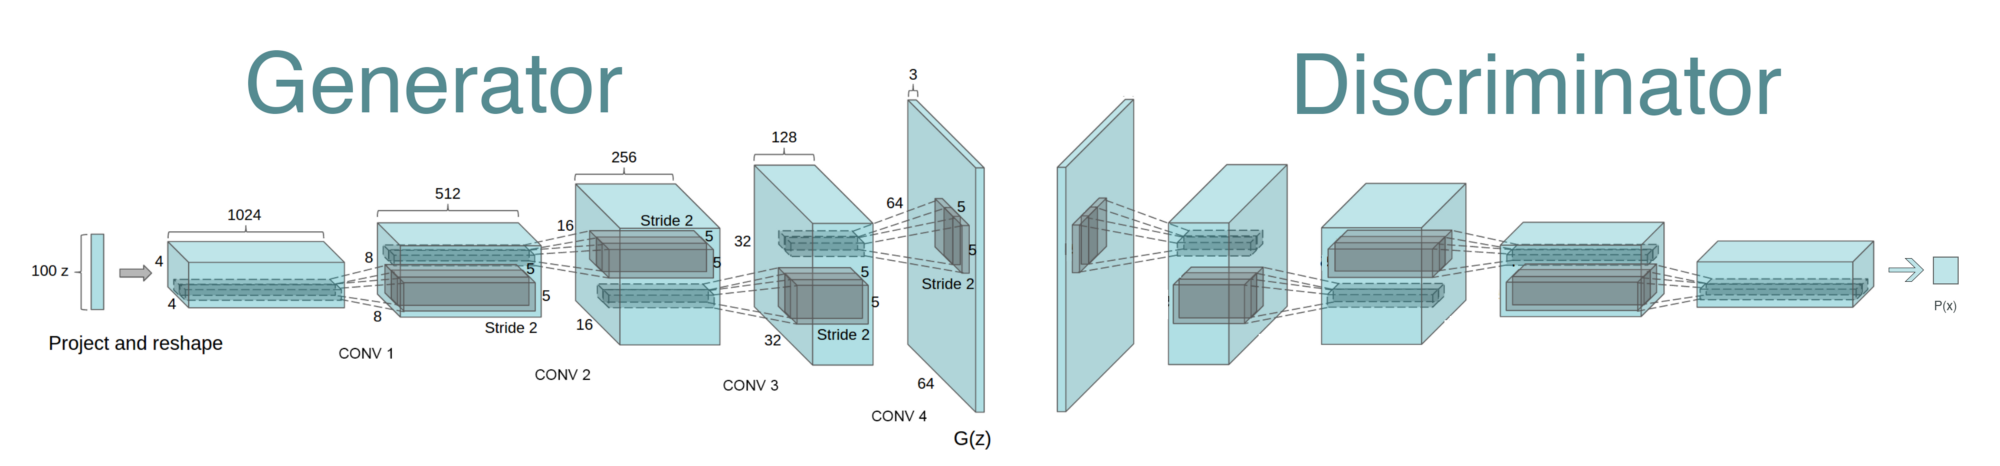
\includegraphics[width=\linewidth,scale=0.1]{figures/1_39Nnni_nhPDaLu9AnTLoWw.png}
  \caption{The network architecture here is a modification of Deep Convolutional GAN (top) consisting of convolutional layers for the discriminator and transposed convolutional layers for the generator.  We modify this by including the auxiliary network of InfoGAN with the Wasserstein objective of WGAN.}
\end{figure}\label{nnet}

\subsection{Network Architecture}\label{arch}
Our network architecture is shown in \label{nnet}.  We employ slight deviations from the DC-GAN paper.  In all layers, we apply batch normalization to prevent saturation of gradients. Weights for each layer are initialized using initialization as proposed by Glorot et al [glorot]. The discriminator network consists of 4 convolution layers with leaky RELU activation in an effort to prevent vanishing gradients as suggested in \cite{Radford2015UnsupervisedNetworks}. By default, we set the size of the kernel in each layer to 3x3, and the double the filter size (number of hidden units) in each subsequent layer by 2 with the exception of the last layer to have a filter size sequence of 32,64,128, and 1028.

	Each convolution layer is followed by a space to depth layer with block size 2.  This is to resize activations between convolutions, transferring height and width data to depth, while retaining all of the data, as opposed to max or sum pooling. That is, given an input of size $ b\times h\times w\times l$ for a minibatch size $b$, the output of this layer of this layer is $b\times h/B \times w/B \times l B^2$.  This is in part because we ideally would like to retain the multipoint statistics of the medium represented by each image.  

	The generator network takes in what is by construction a 1 dimensional entity consisting of random code values sampled according to a chosen distribution.  Since the generated data will in essence be at some level described by a distribution more complicated than a set of univariate standard Gaussians, we pass these first through a nonlinear fully connected layer with, for a single channel image, 1024 hidden units and Relu activation.  The output of this first layer is reshaped to a 4D tensor of size $b\times d_z \times d_z \times 256$ and passed through 4 strided transpose convolution layers with, for a single channel image, filter sizes 128, 64, 32, and 1 respectively.  Following each of these  strided transpose convolution layers is a depth to space transformation with block size $2$ to resize outputs of hidden layers without averaging retaining information by max-pooling.  The input values of the random code are drawn from a distribution that can be specified from among uniform, truncated normal, or normal.  As described in \cite{Tipping1999ProbabilisticAnalysis} by Tipping and Bishop, the probabilistic interpretation of PCA shows that the coefficients in the Principal component basis are normally distributed and uncorrelated.  Hence, we extend the number of possible distributions to include the principal components of some associated data.  We discuss later the impact of drawing from the principal components associated with the training data.

	We replace the original or heuristic objectives of the GAN with that used in \cite{Arjovsky2017WassersteinGAN} for the WGAN architecture, the approximate Wasserstein metric, while also clipping the weights of the discriminator.  As was done in \cite{Chen2016InfoGAN:Nets}, within the discriminator we include layers for an auxiliary network to update latent variables $c$ associated with the variational upper bound described in InfoGAN.  We assume, as the authors in [InfoGAN] did, that the additive constant entropy function of the latent variables is constant.
    
	We employ Adam optimization for the generator, discriminator, and auxiliary network for a pre-specified number of discrete and continuous latent variables.  We employ Tensorflow's exponential moving average functionality to maintain moving averages of weights/training variables by employing an exponential decay, as this has been shown to be beneficial for training.
    
Specifically, regarding optimization objectives we first recall WGAN. In place of single probabilities, with the vision of Arjovsky, we consider instead distributions describing the authenticity of data. Given probability distributions $P_r $ corresponding to real data and 
$P_g $ corresponding to generated data, the Wasserstein Metric--also known as the Earth Mover Distance--is defined as
\[
W(P_r,P_g) = \textbf{inf}{\gamma \in pi(P_r ,P_g)} \mathbb{E}_{(x, y) \sim \gamma} |x - y|
\]

Where $ \Pi(P_r,P_g) $ denotes the set of all joint distributions whose marginals are $P_r$ and $P_g$.  As defined, this computation is intractable.   Rubinstein-Kantorovich Duality implies that:
  
\[
W(P_r,P_\theta ) = \sup_{|f|_L \leq 1} \mathbb{E}_{x\sim P_r}[f(x)] - \mathbb{E}_{x \sim P_\theta}[f(x)] 
\]

Which can be evaluated without a function $f $ by confining the updates of $ W $ to a compact set through weight clipping.  While gradients may vanish in this fashion, we experienced no such issue with the dataset. 

The auxiliary network defined within the Discriminator takes as input (in original GAN) the penultimate  layer of the discriminator, that preceding the sigmoid layer. This can be interpreted as the discrete probability density of authenticity as in WGAN.  There are a finite number of categories, so we compute from the categorical input layer a softmax activation.  The outputs of the second layer corresponding to sets of continuous random variables is a hyperbolic tangent nonlinearity.  The objective is simply the mean over all continuous latent variables summed with the total entropy of the categorical variables.

By contrast with ALI, we hope to perform a more efficient, though less general, operation mapping physical data to GAN reconstructions with the aim of identifying similar generated images to the input.  The idea is that, if the images for different latent variable values are in some sense similar to the physical image, these generated data can then be used to form a closed form representation of the principal component basis furnished by the discrete KL transform (PCA).  We show results for the method in the Evaluation section \label{evaluation}, but find that the latent variables trained are sufficiently representative to allow us to disregard this approach. 


\section{Evaluation (synthetic and real data and comparison to baseline and other methods)}\label{evaluation}

In place of a synthetic set of data, we train our model on both the MNIST digits in an unsupervised fashion, as well as the $32\times 32$ pixel images of channelized media described in the previous section \label{related}.  In all cases, we use a mini-batch size of $64$ samples while varying the number of categorical and continuous variables (see attached results figures).

Consider the loss \label{MNISTt} and generated images \label{MNISTg} produced by training the model using MNIST, specifying 10 latent categories and 2 continuous transformations.  We observe that the loss function seems to converge quickly, and the generator yields fascinating representations for two categories.  In particular, we seem to have formed a new category (corresponding to Greek lambda).  Other learned categories are not necessarily correct, either.  This may be due to early stopping of the training at 2000 iterations.

\begin{figure}[h]
% \centering
  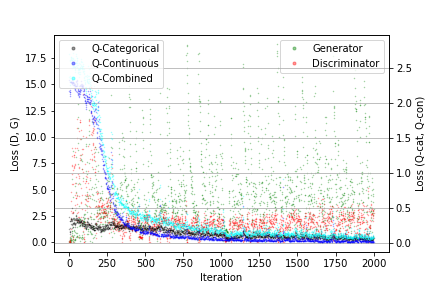
\includegraphics[]{figures/lPlotGDQQData2Axes.png}
  \caption{Generations using 10 latent categories and 2 continuous latent variables for the MNIST Data. }
\end{figure}\label{MNISTt}

\begin{figure}[h]
% \centering
  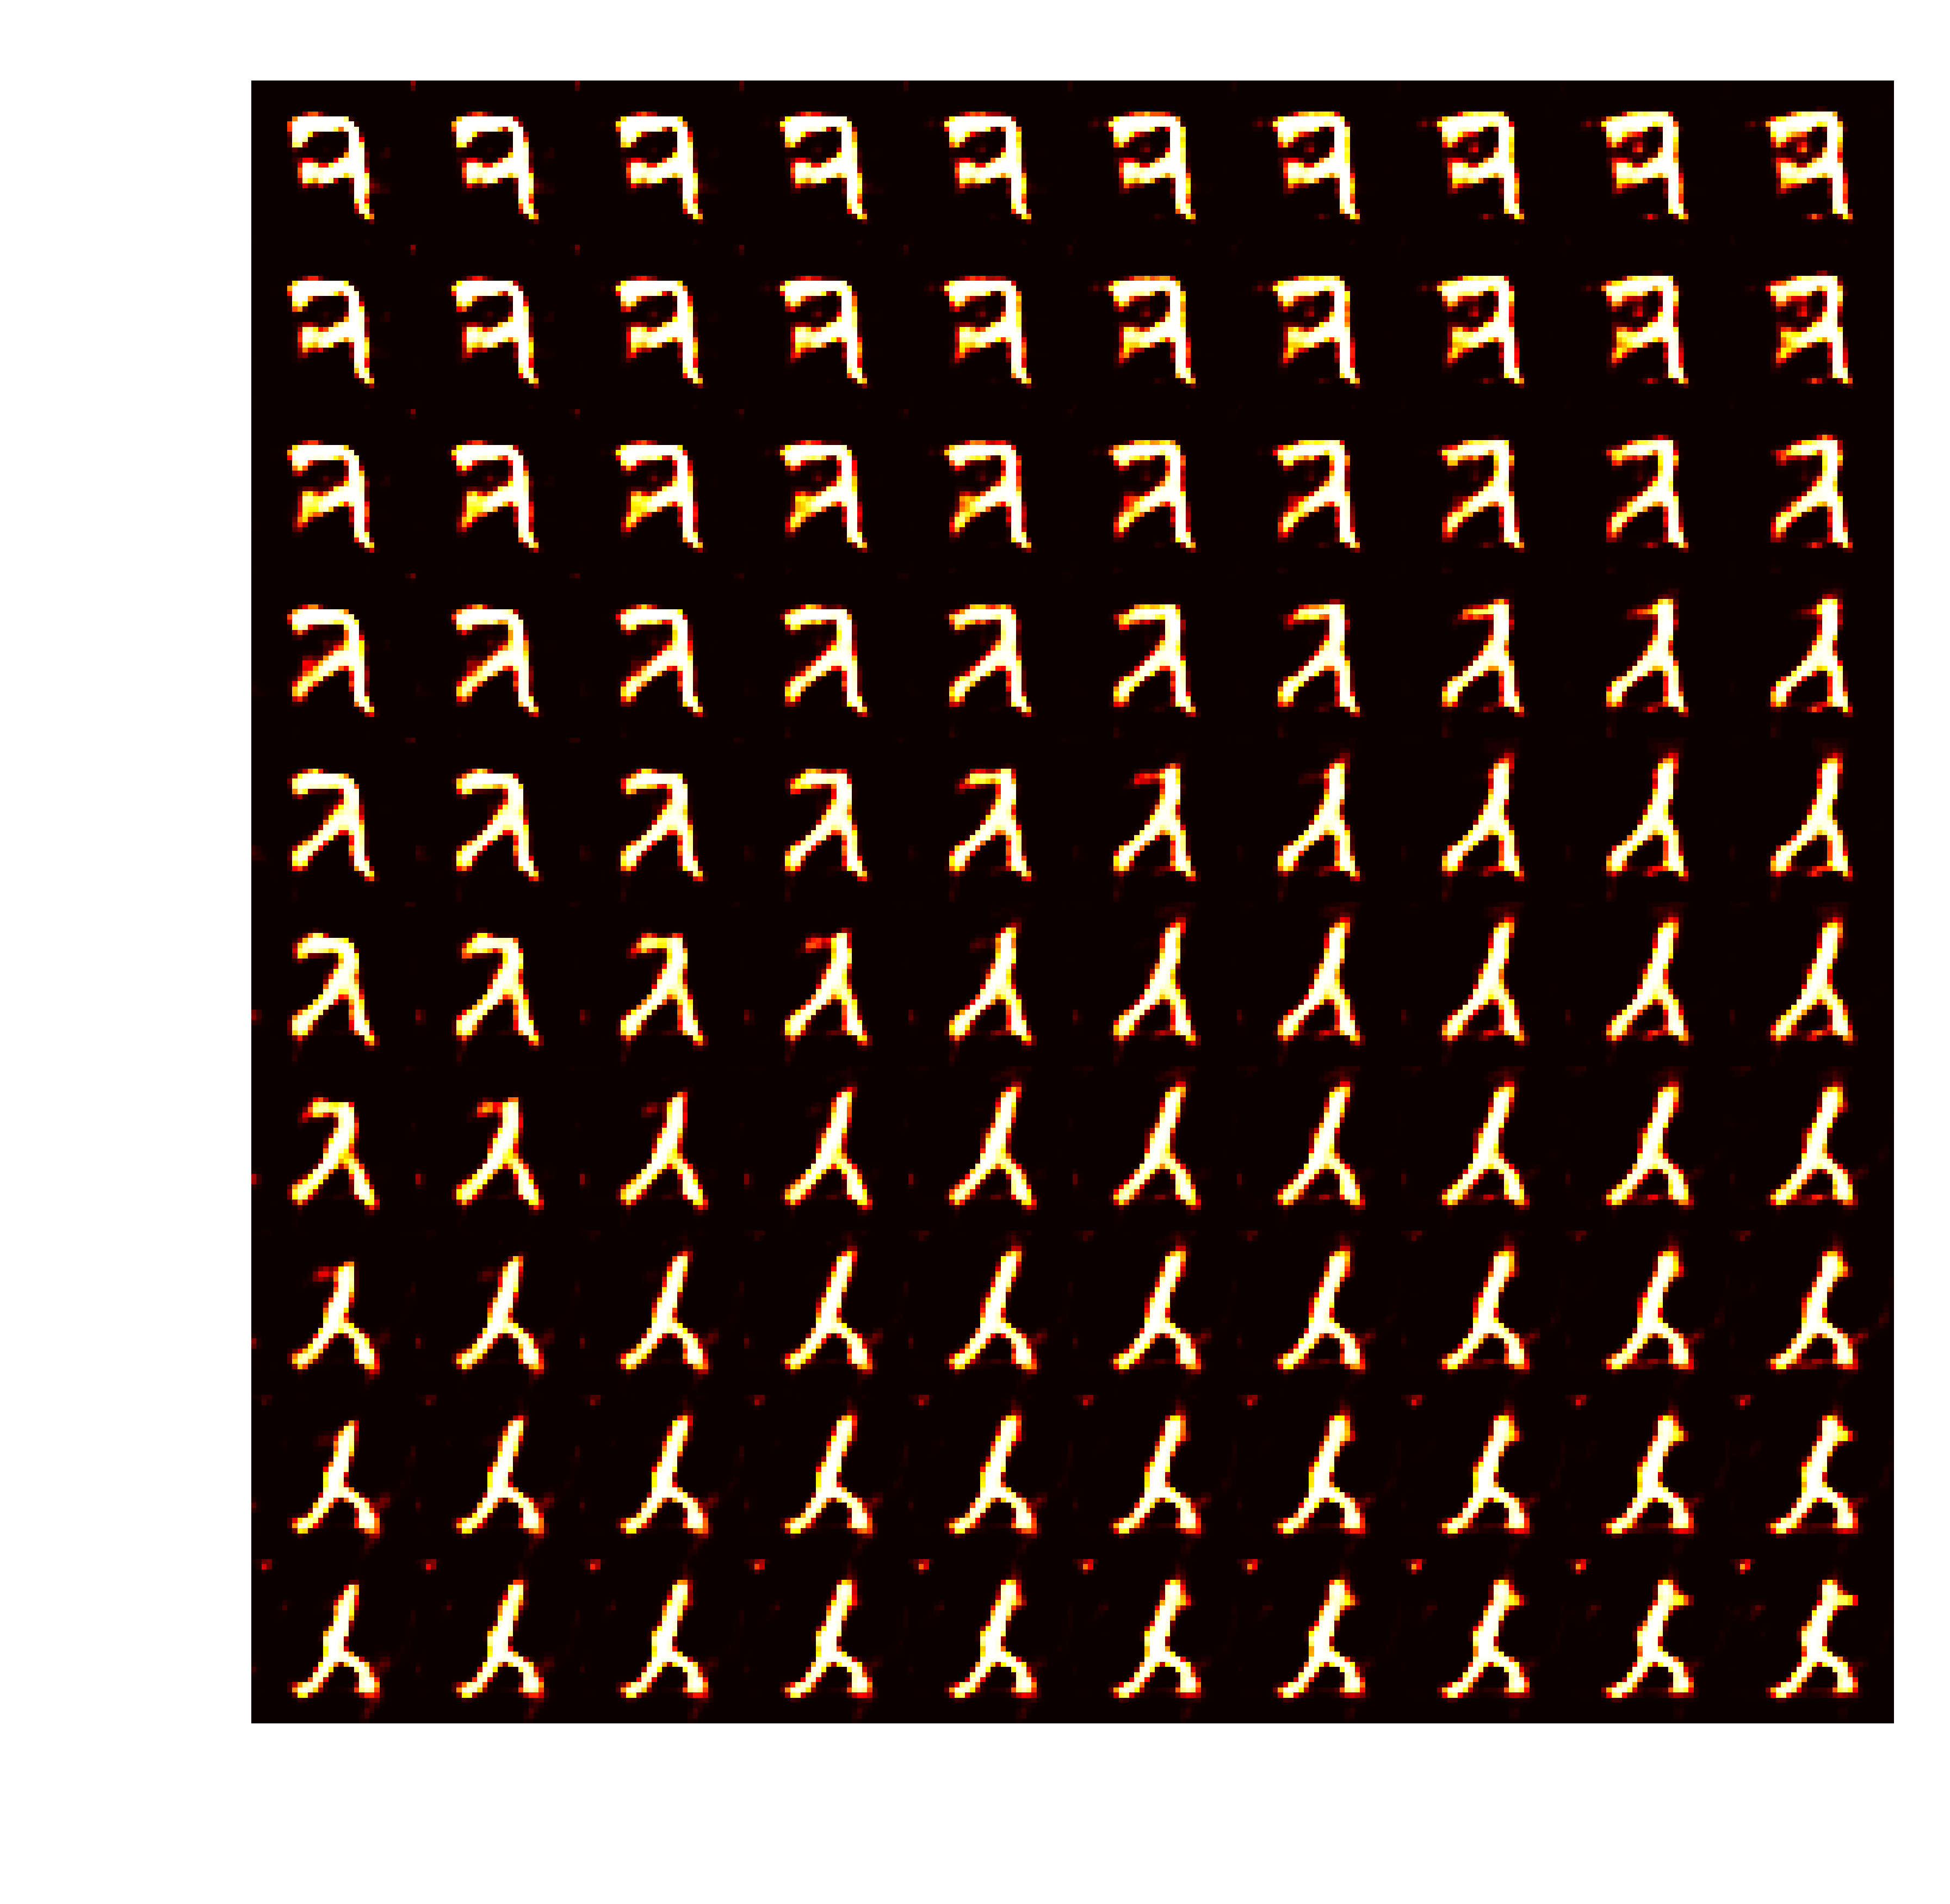
\includegraphics[scale=0.1]{figures/samples_zk_6.png}
  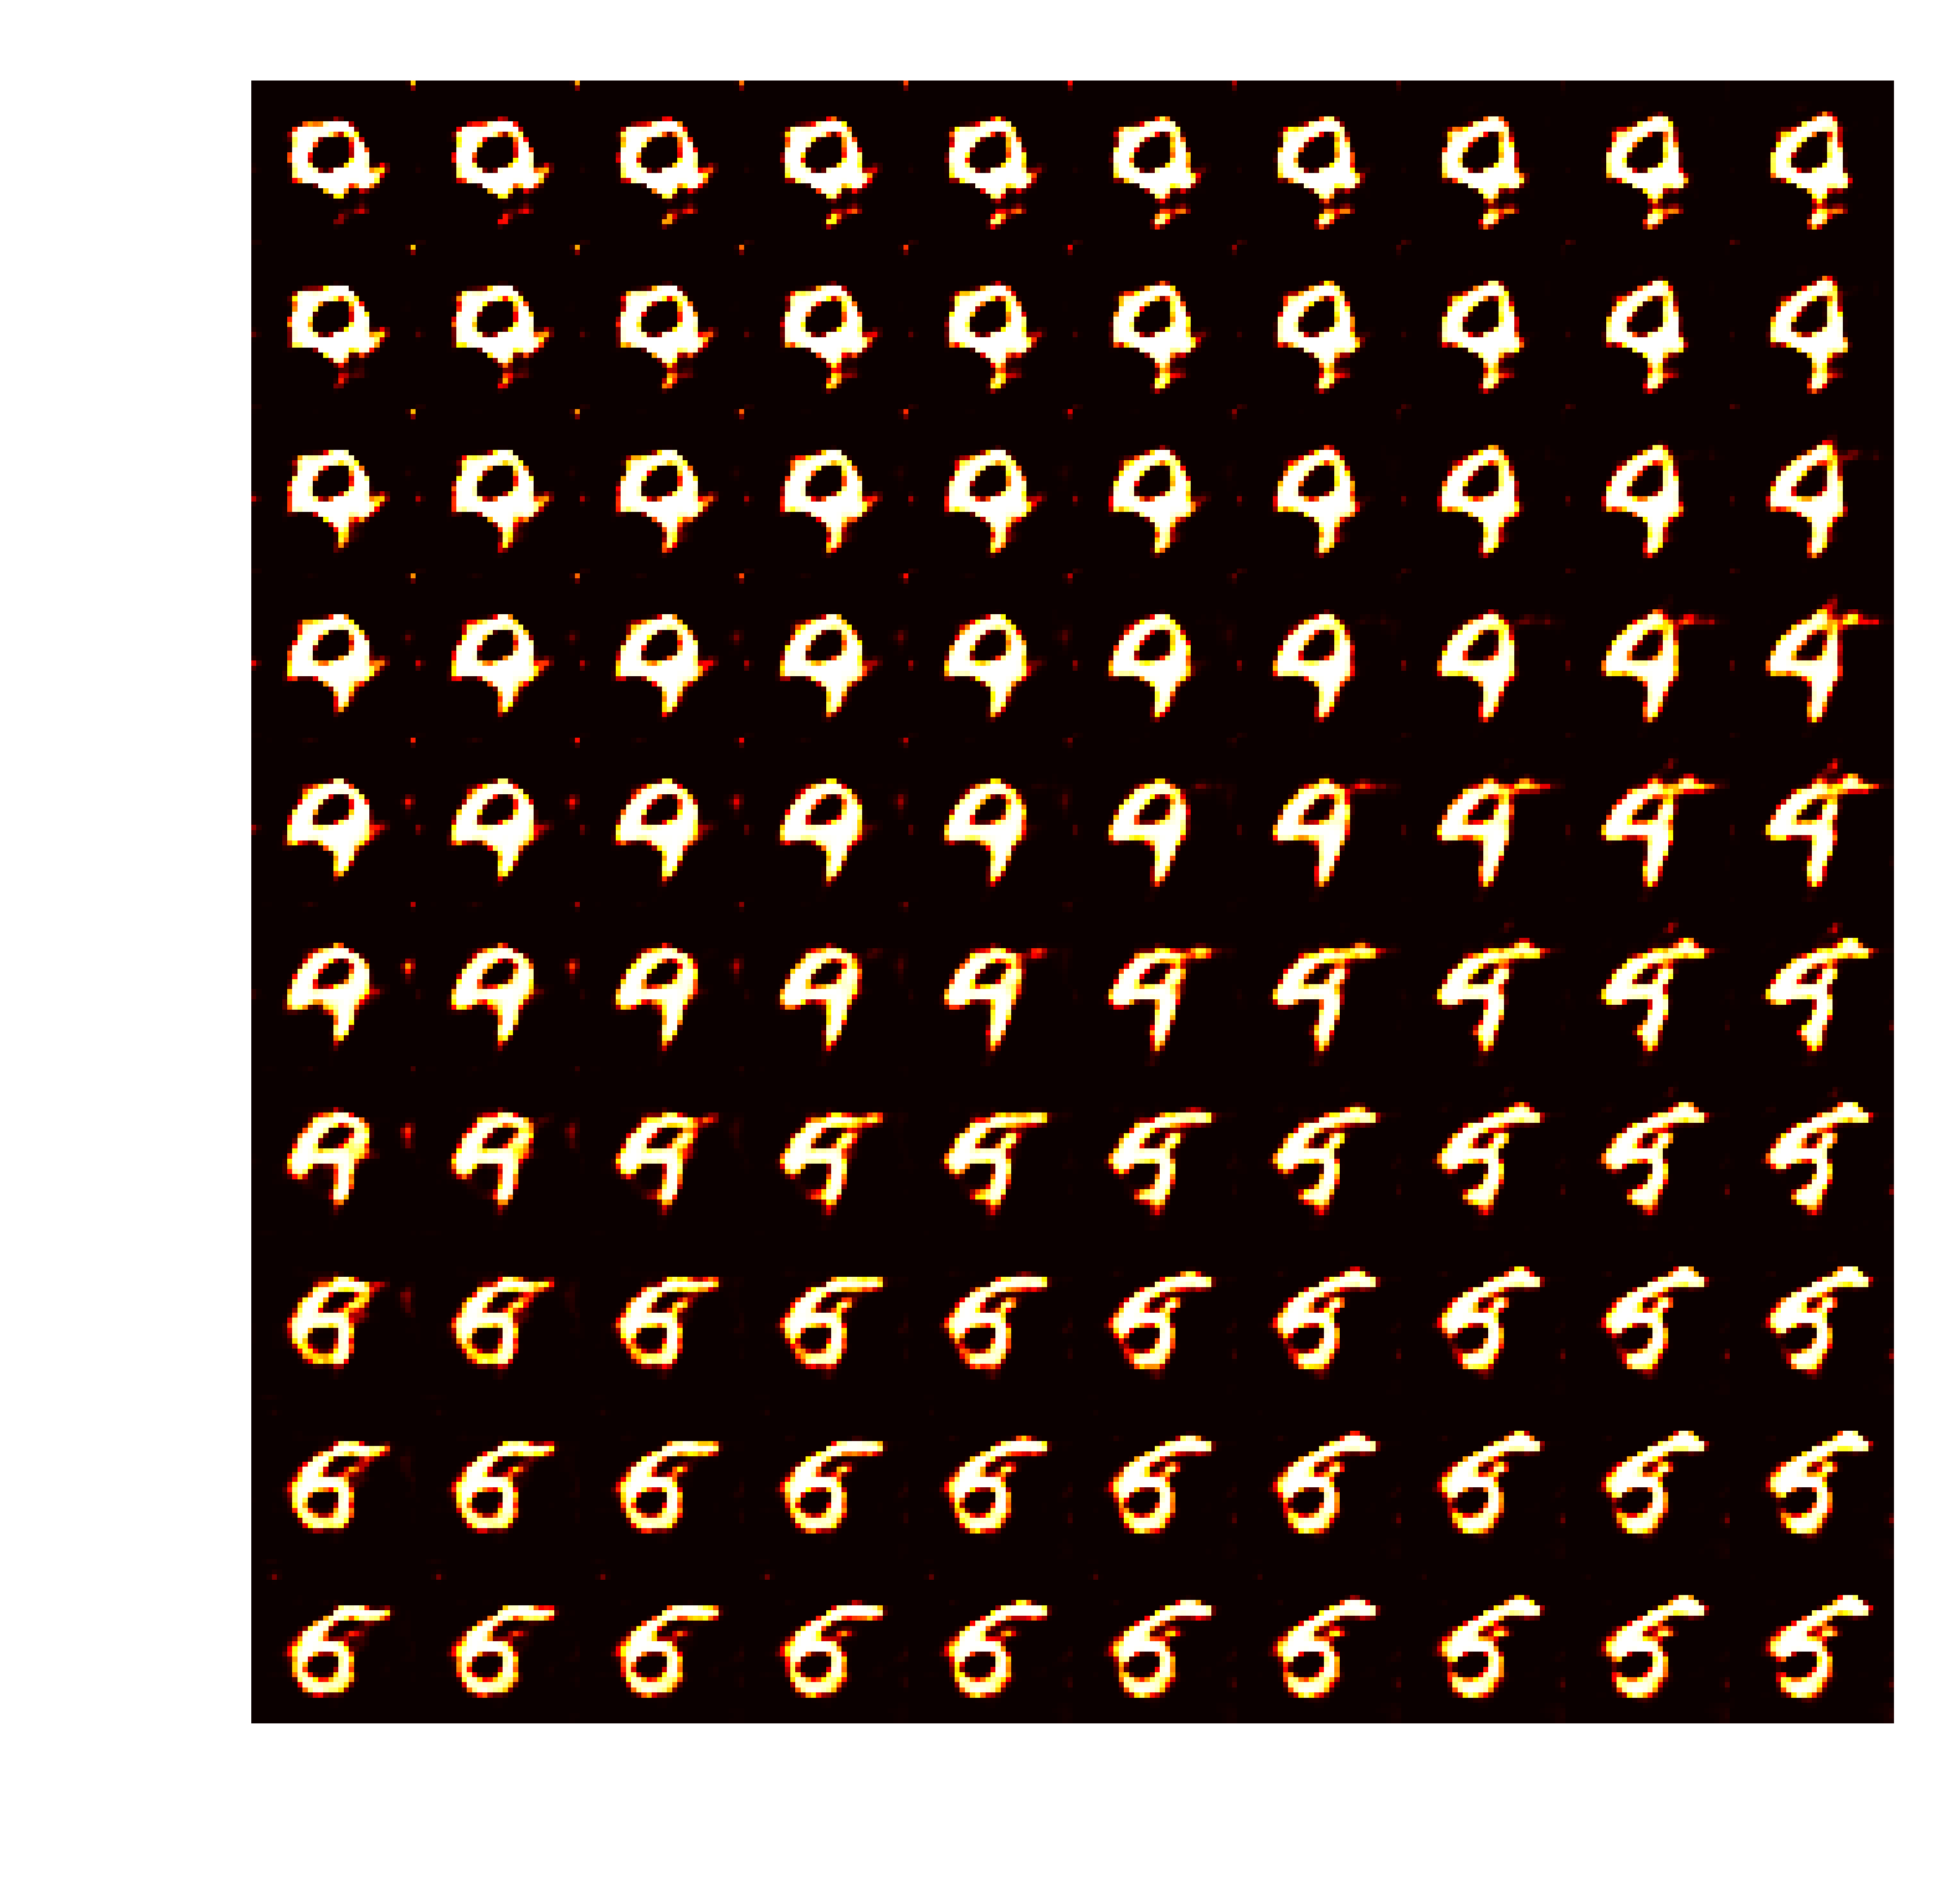
\includegraphics[scale=0.1]{figures/samples_zk_7.png}
  \caption{Generations using 10 latent categories, with two depicted: $5$ (top) and $6$ (bottom). and 2 continuous latent variables for the MNIST Data.}
\end{figure}\label{MNISTg}

For the network using design elements from both InfoGAN and WGAN, we vary the dimensionality (number of independent) random codes used to sample as in the original GAN formulation, and find that the model is insensitive to their number, given a nontrivial number of categories (for example, 4 categorical and 2 continuous).

First, as a test of our idea to associate training data images with network generations, we observe the impact of determining the principal component decomposition in terms of a number of modes equal to the dimensionality of independent random codes to be sampled.  We begin with elements of InfoGAN alone, optimizing with respect to the stabilizing heuristic with a change of minimizing $\log(1-p_G)$ to maximizing $-\log(p_G)$. Consider figure \label{mapPCA}, where we plot the results of training this simpler network without WGAN influence.  We see that the reconstruction (top) is nearly indistinguishable from the generated data using fixed samples of the PC components of training data.

\begin{figure}[h]
  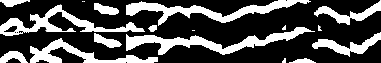
\includegraphics[]{figures/pcamap.png}
  \caption{ (Top) Generative Reconstruction using coefficients of PCA for random noise variables as generator input.  Reconstructions learned by a Variational Autoencoder, which takes approximately 10 minutes to train for 2000 iterations on the same data, compared with 1 minute for the GAN constructed here.}
\end{figure}\label{mapPCA}

Consider Figure \label{zPCA}, where the loss of each network is plotted.  These losses correspond to a model where, at each training iteration, samples of noise $z$ are not random, but instead are conditioned on the PC coefficients of the training data in the current batch. We observe strange behavior, as one might expect, since these are not random samples, but are conditioned on the data in the minibatch (and, possibly, the entire dataset, as the SVD is taken prior to training in this case).  While generated samples seem to exhibit the continuity of change in latent variables, we examine a related distribution to test if this is a result of conditioning.  In \label{tnorm}, we see that samples of a truncated normal lead to the same result.  So the sampled distribution can have an observable influence on the results, as, for example, we see in these case the categorical distribution no longer decays to $0$.  In any case, we do determine a mapping from samples in each batch to generated images using the trained model, though we do not make use of it, as our primary goal is in unsupervised learning using the GAN to furnish a useful basis for determining smooth transformations of complex data (in part to find nearest neighbor using an implicitly learned similarity metric).
Ultimately, we see that the noise variables sampled from a uniform distribution yield clear decay of the loss of the Q-network.

\begin{figure}[h]
% \centering
  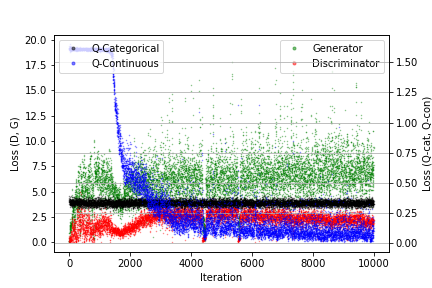
\includegraphics[]{figures/Sampling_PCA.png}
  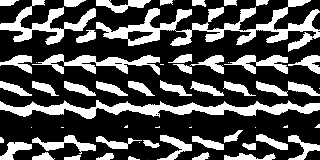
\includegraphics[]{figures/PCAsample_fig_test.png}
  \caption{Loss (top) of each network corresponding to a model where, at each training iteration, samples of noise $z$ are not random, but instead are conditioned on the coefficients of the training data in the Principal Component Basis.  Generations (bottom) from the trained network.}
\end{figure}\label{zPCA}

\begin{figure}[h]
% \centering
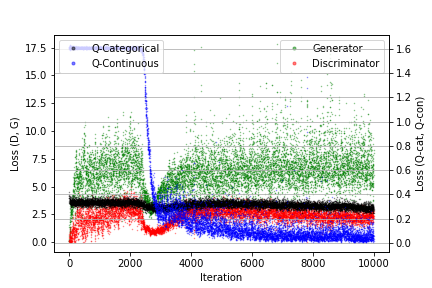
\includegraphics[width=\textwidth,scale=0.1]{figures/SampleTruncNorm.png}
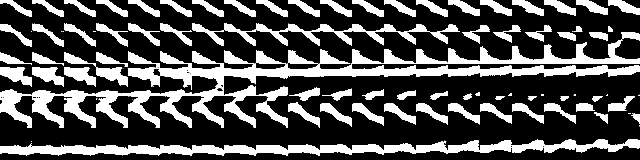
\includegraphics[width=\textwidth,scale=0.1]{figures/Sample_TruncNorm.png}
  \caption{Results for training loss history(top) and resulting snapshots in the case where random noise is sampled from a truncated standard normal.  }
\end{figure}\label{tnorm}


\begin{figure}[h]
% \centering
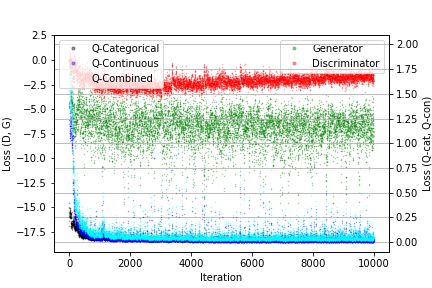
\includegraphics[width=\textwidth,scale=0.1]{figures/Sample_Uniform.png}
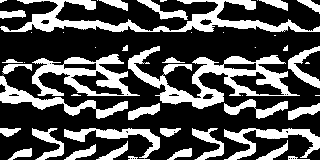
\includegraphics[width=\textwidth,scale=0.1]{figures/SampleUnifTest.png}
  \caption{Losses resulting from sampling noise variables from a centered uniform distribution from $-1$ to $1$ }
\end{figure}

We now consider, as alluded to in our Description of the model, a set of realizations of the medium of higher dimensionality/with a larger number of features, $d=4096$ ($64\times64$, when considered as images) so as to be able to split the data while retaining a meaningful number of samples.  Results using this higher-dimensional dataset consisting of $200,000$ training images is shown in \label{GenPCA2}.  

\begin{figure}[h]
% \centering
  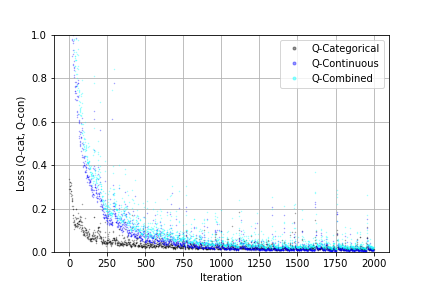
\includegraphics[width=\textwidth,scale=0.2]{figures/PlotQQData2Axes_ylim.png}
  \caption{Value of loss corresponding to the categorical, continuous, and combined loss of the auxiliary network maximizing mutual information between latent variables in the variational upper bound associated with the InfoGAN component of the network. Training and validation data correspond to larger images of size $64 \times 64$ as generated by the SNESIM algorithm, reduced from larger images to incorporate horizontal and vertical shifts of realizations in the training data.  The loss converges rapidly for both within a small number of iterations.  We see no significant difference between validation and training error, suggesting that we are not experiencing over-fitting.}
\end{figure}\label{GenPCA2}

\begin{figure}[h]
% \centering
  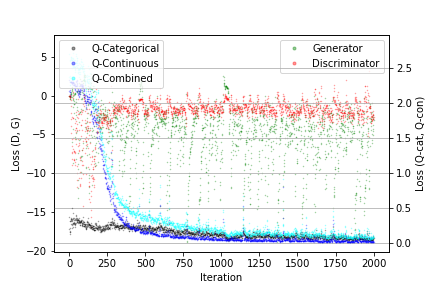
\includegraphics[width=\textwidth,scale=0.2]{figures/PlotGDQQData2Axes.png}
  \caption{Values of the losses associated with the Discriminator and Generator for the training and validation data.  The case corresponds to the optimal case described above.  There is a high variation in the generator, and the low variation in the discriminator.  From previous results (see included figures), it seems that, when the latent variables in the auxiliary network have converged (as happens rapidly in all cases), the primary influence on the weights of the generator results from changes in data between minibatches due to the sheer amount of training data (approximately $200,000$ samples).  Also, inherently random samples of (meaningless) codes, remnants of the original GAN, may influence updates in the weights once assignments latent variables have to some extent converged.}
\end{figure}\label{}


\begin{figure}[h]
% \centering
  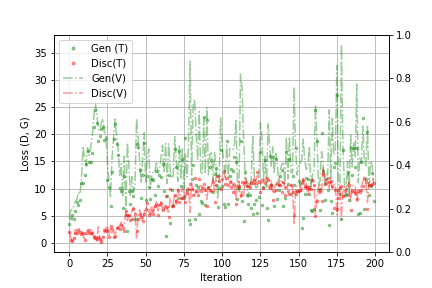
\includegraphics[width=\textwidth,scale=0.2]{figures/PlotGDData2Axes_Train_Validation_GD.png}
  \caption{Value of loss corresponding to the categorical, continuous, and combined loss of the auxiliary network maximizing mutual information between latent variables in the variational upper bound associated with the InfoGAN component of the network.  Here the model learns 6 categories of images and 2 continuous transformations of the data. Please see Discussion.}
\end{figure}\label{cat6gd}

\begin{figure}[h]
% \centering
  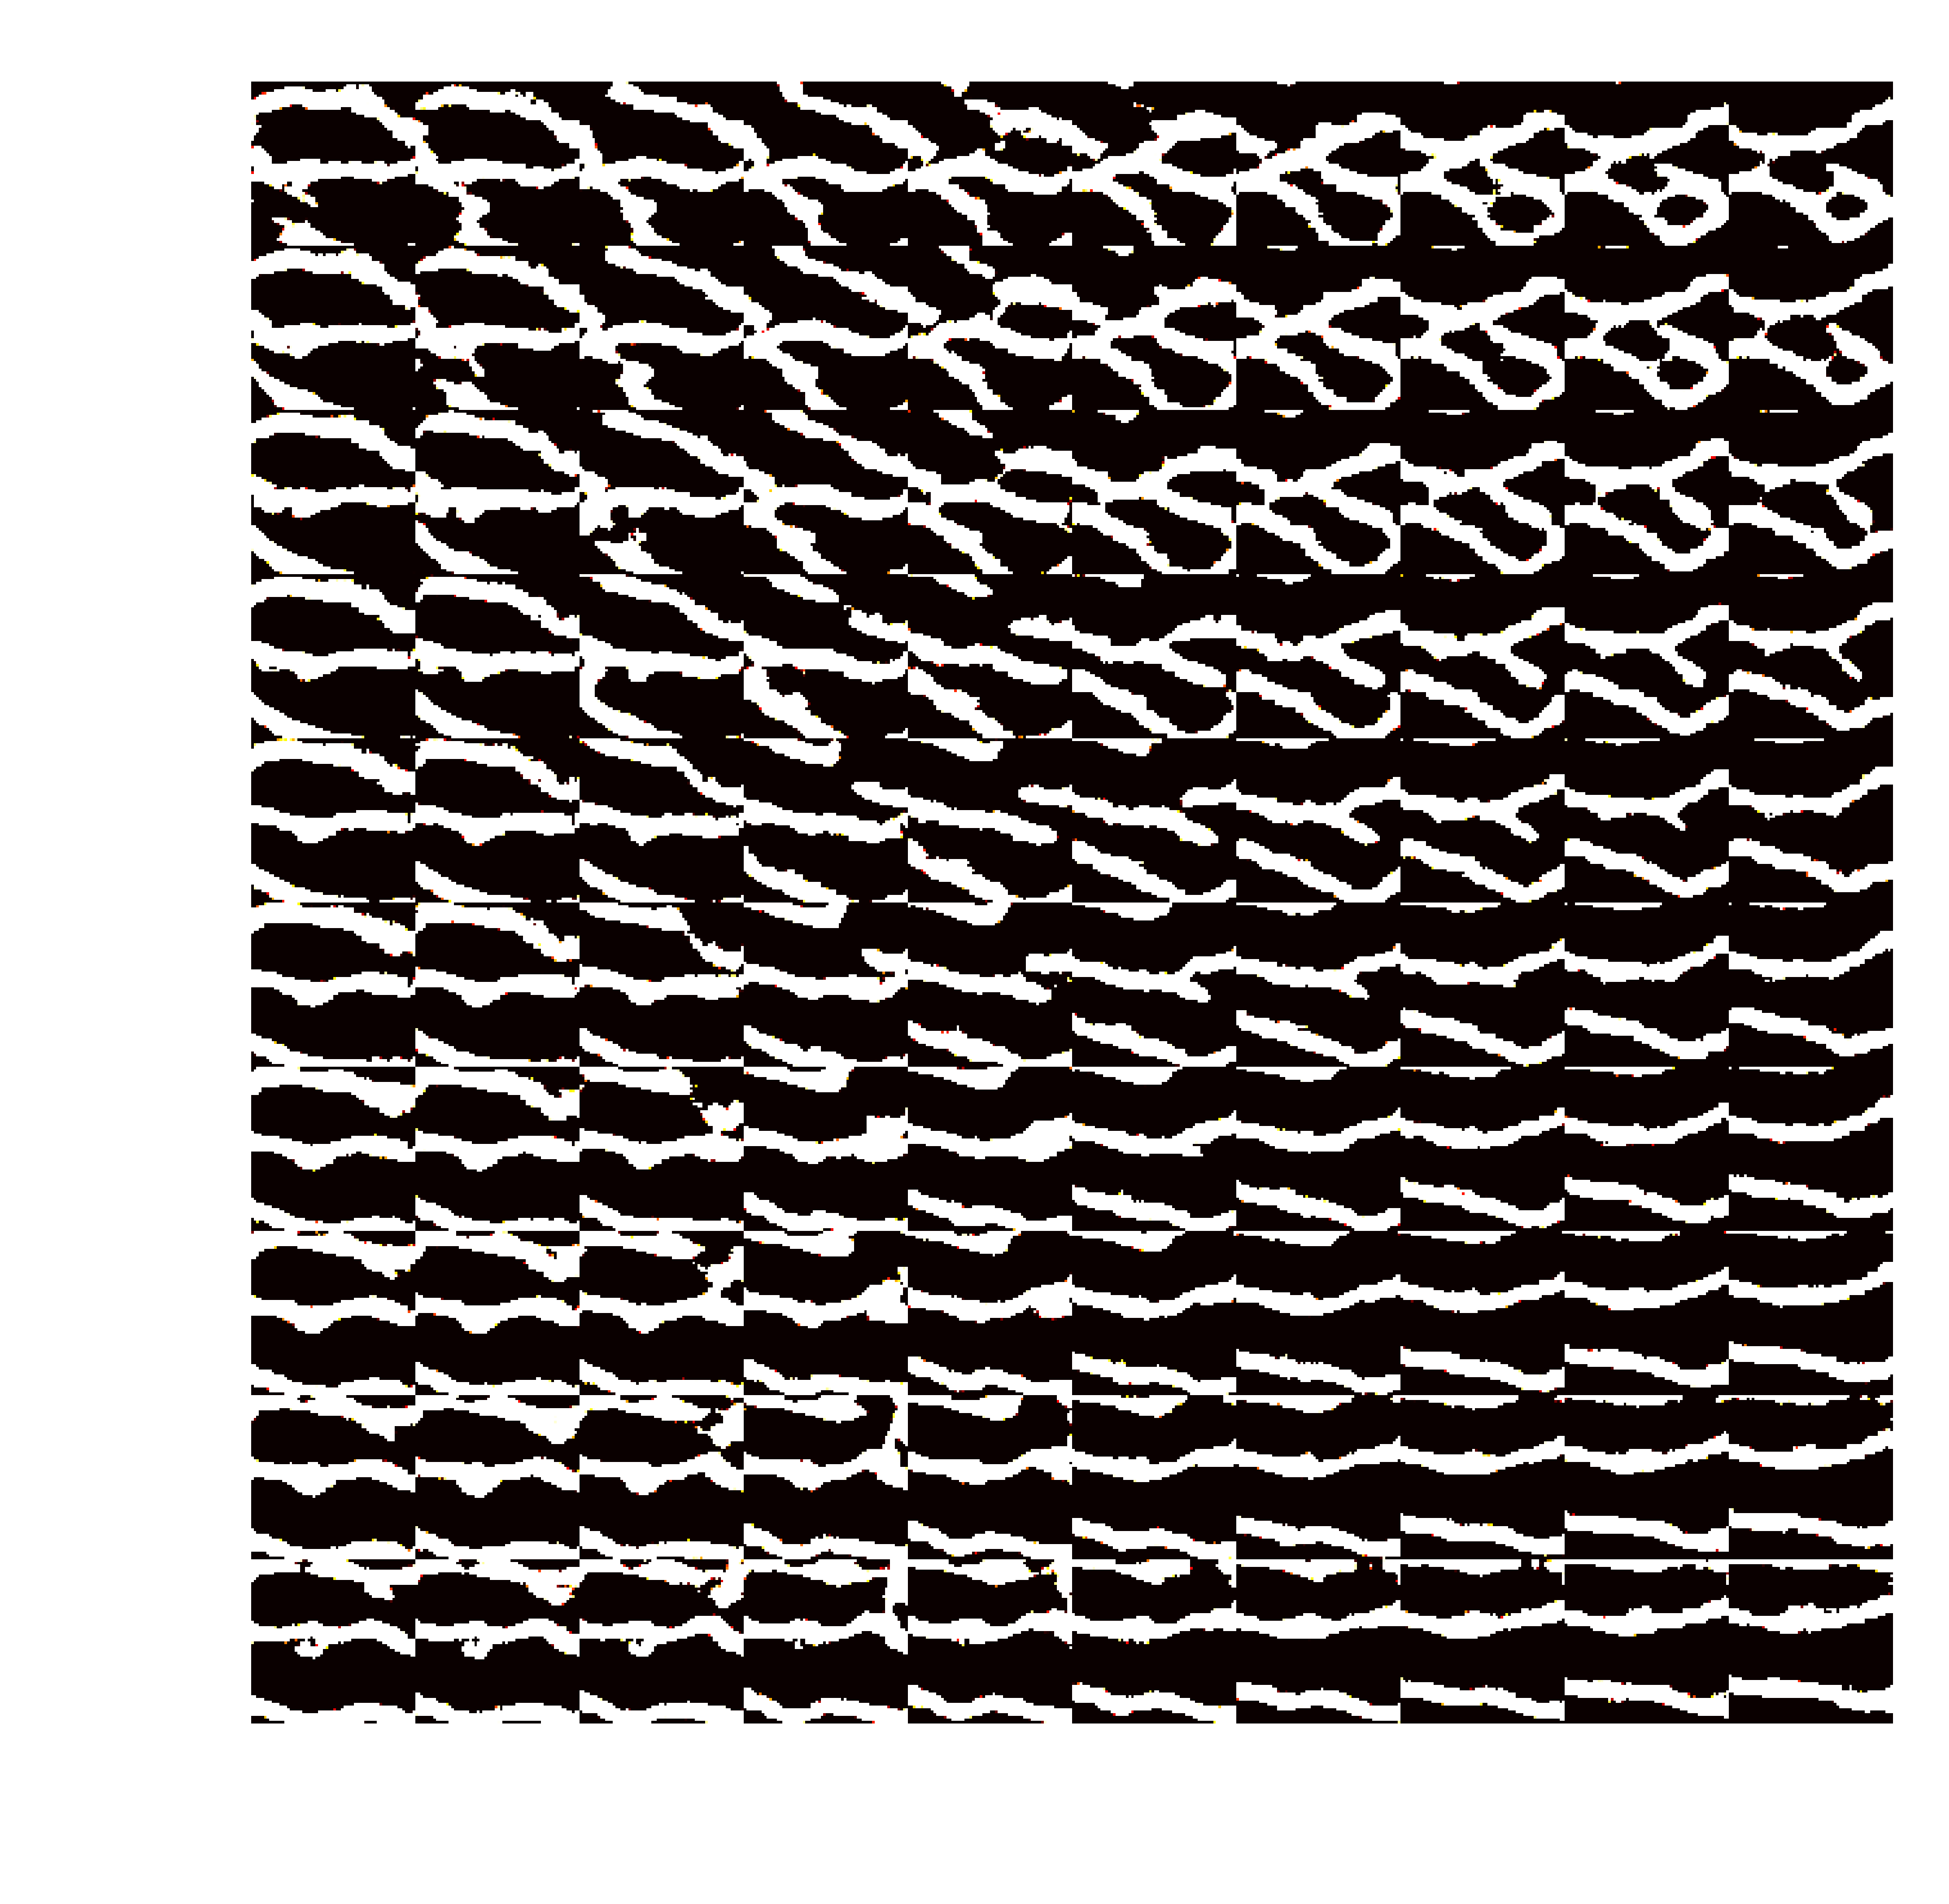
\includegraphics[width=\textwidth,scale=0.2]{figures/samples_zk_0.png}
  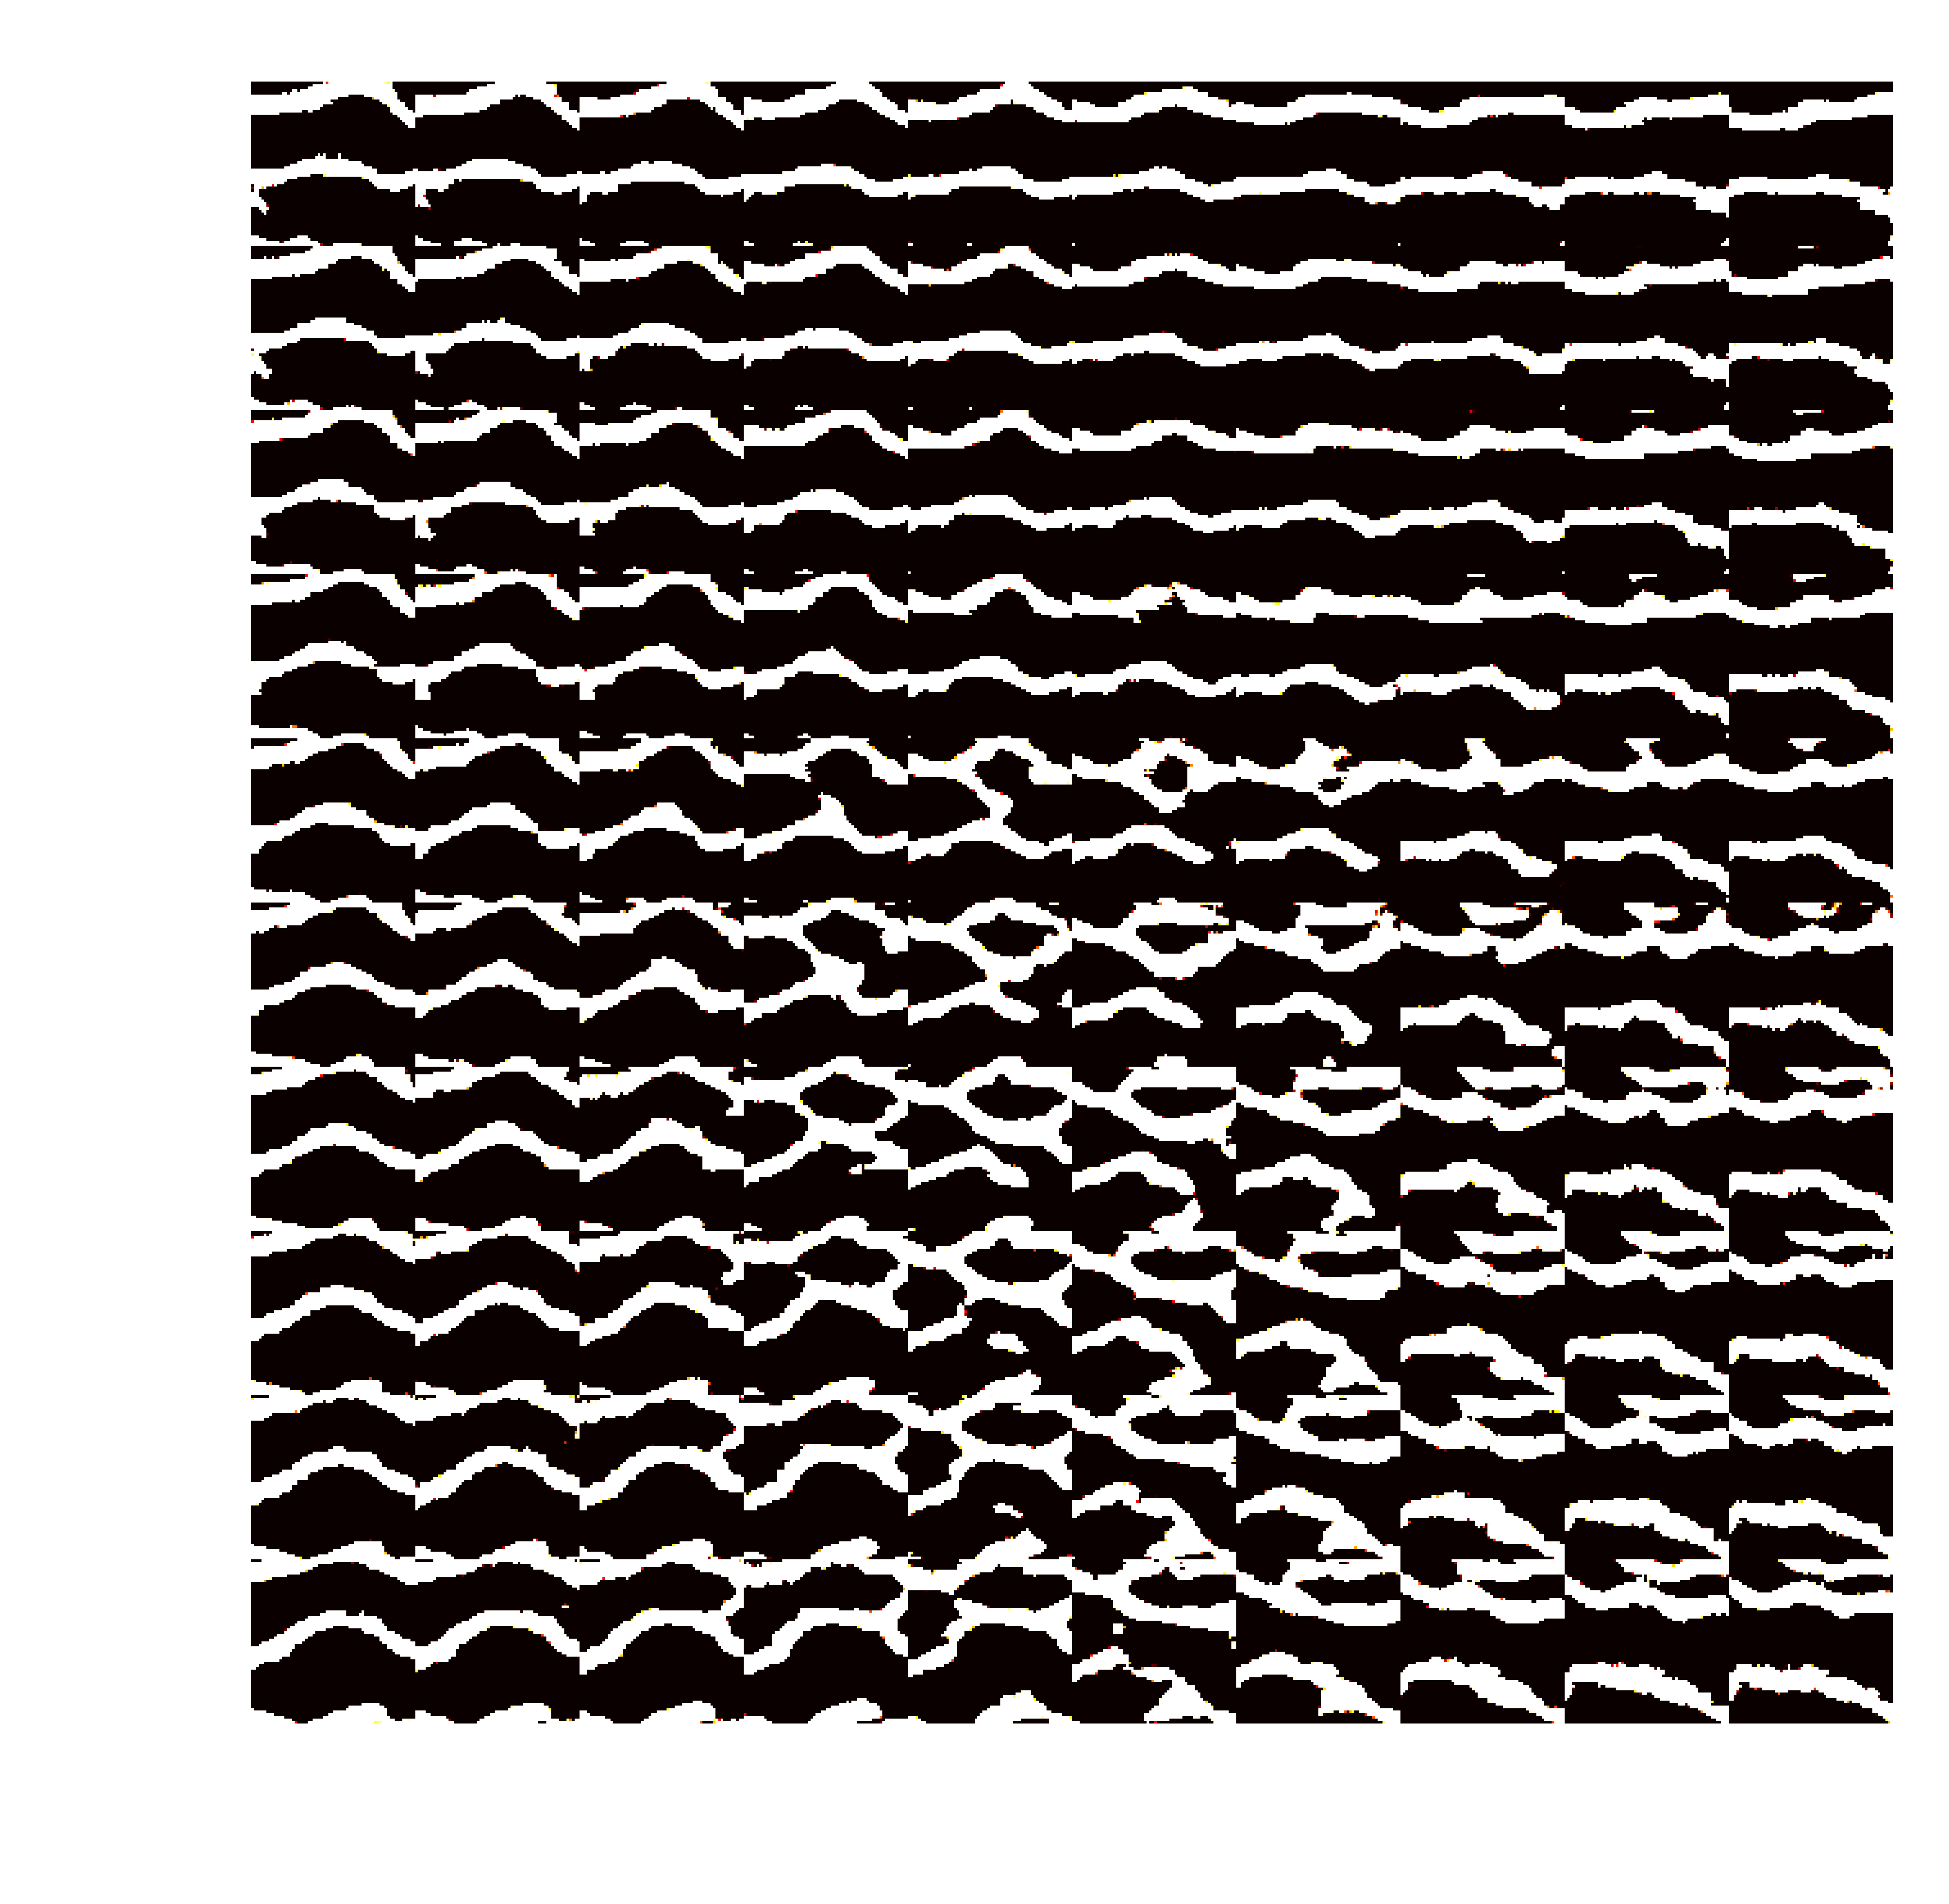
\includegraphics[width=\textwidth,scale=0.2]{figures/samples_zk_5.png}
  \caption{Images generated following training using a uniform mesh created from values of the  two continuous latent variables from $-1$ to $1$.  The model corresponds to $6$ values of the categorical values.  Transformations between images visually continuous within both categories $0$ (top) and $5$ (bottom). Please see Discussion.}
\end{figure}\label{cat6samples}

\begin{table}[t]
  \caption{Mean Value of Latent Variables}
  \label{sample-table}
%   \centering
  \begin{tabular}{lll}
    \toprule
    \multicolumn{2}{c}{Part}                   \\
    \cmidrule{1-2}
    Data       & Continuous      & Categorical \\
    \midrule
    Training   & $[ 0.02 -0.01]$ &$[ 0.19  0.07  0.08  0.48  0.07  0.10 ]$ \\
    Validation & $[-0.11  0.20]$ & $[ 0.01  0.74  0.03  0.08  0.07  0.056]$     \\
    Test       & $[ 0.45 -0.06]$       & $[  0.000516   .002   0.0007   .099 0.00172   0.000706 .004]$  \\
    \bottomrule
  \end{tabular}
  \caption{Table of mean values of the auxiliary $Q$ distribution of the trained network. While sampled means are quantitatively distinct, Qualitatively, one may observe that, for example, the training and test data both find a maximum value in Category 3.  One factor influencing this result is that the Training data have been preprocessed, making them unsuitable as a basis of comparison.  The number of test samples in this case is much smaller than either validation or training samples.}
\end{table}

% The reader is asked to please see the attached figures for more results in this and other cases. Sample generation took on the order of seconds over all categories. With these results, it is clear that, given an image of interest, one may use the trained model to project--through the auxiliary network defined within the discriminator--the data to its associated latent categorical and continuous coordinates.  With this reduced representation, arbitrarily many samples for nearby continuous values within the fixed category determined for the sample can be generated.  These generated or 'surrogate' realizations representing continuous transformations of an image (of the channelized medium) of interest can then be used to form a dataset conditioned on a single sample or subset of the original data.  This conditioned, surrogate dataset with arbitrarily many samples can then be used to furnish a basis using a dimensionality reduction technique such as Linear or Kernel PCA that furnishes a basis that not only is representative of the data, but captures smooth deformations in the structure of the data





\section{Discussion}

	Consider \label{cat6samples}, which showcases results from varying the number of categories from $4$ to $16$ suggest that 2 continuous transformations are best observed qualitatively for $6$ possible values of a single categorical latent variable.  Training and validation data correspond to larger images of size $64 \times 64$ as generated by the SNESIM algorithm, reduced from larger images to incorporate horizontal and vertical shifts of realizations in the training data.  The loss converges rapidly for both within a small number of iterations.  We see no significant difference between validation and training error, suggesting that we are not experiencing over-fitting.

	Consider \label{cat6gd} in the previous section, displaying images generated following training using a uniform mesh created from values of the  two continuous latent variables from $-1$ to $1$.  The model corresponds to $6$ values of the categorical values.  Transformations between images visually continuous within both categories $0$ (top) and $5$ (bottom).  The reader is asked to please see the attached figures for more results in this and other cases. Sample generation took on the order of seconds over all categories. 
    With these results, it is clear that, given an image of interest, one may use the trained model to project--through the auxiliary network defined within the discriminator--the data to its associated latent categorical and continuous coordinates.  With this reduced representation, arbitrarily many samples for nearby continuous values within the fixed category determined for the sample can be generated.  These generated or 'surrogate' realizations representing continuous transformations of an image (of the channelized medium) of interest can then be used to form a dataset conditioned on a single sample or subset of the original data.  This conditioned, surrogate dataset with arbitrarily many samples can then be used to furnish a basis using a dimensionality reduction technique such as Linear or Kernel PCA that furnishes a basis that not only is representative of the data, but captures smooth deformations in the structure of the data. 
    
	We demonstrate the above, and apply the proposed method by using the trained network to generate $2500$ samples, varying only one latent parameter to obtain a sequence of images corresponding to continuous deformations of the original channelized medium.   the figure of samples using KDE and PCA from the proposed model at the beginning of this report, which we repeat and extend in this section in Figure [\label{GenPCA2}].  We display the results for the application of PCA to $2500$ generated samples corresponding to a fixed category, fixed random noise sample, varying a single continuous latent variaable. Displayed are the Principal Modes (top), Joint Density of first two principal modes (upper middle), Realizations resulting from Kernel Density Estimation of the principal component basis.  Distribution of errors in KDE-sampled generations for increasing sample size.  We observe that the density of coefficients in the Principal Component Basis is, itself, arguably non-Gaussian as sampled.  Principal modes are all qualitatively similar to a single output of the generator, capturing increasingly finer fluctuations in the basis. This was in large part the objective of the entire procedure.  By restricting the dataset to contain structurally similar data, one essentially forces fine variations to contribute to the the majority of the variance.  Ultimately, this allows for smooth, linear transformations between complex, high dimensional deformations of a given image.
    
    While we have not demonstrated the application in (Weighted) KPCA-based optimization using the Adjoint Method here, it is clear how one would proceed.  Without additional information, one could randomly sample latent variable values to generate realizations of channelized medium, and use these as inputs to the forward model of the inverse problem. One could use any one among a number of methods (Gaussian Process Regression, MCMC) to determine a distribution of latent variable values minimizing the cost, and finally proceed with Kernel PCA-based optimization using adjoint gradients, now with a basis representative of the deformation one wishes to invert.
  
\begin{figure}[h]
\centering
  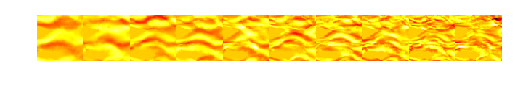
\includegraphics[]{figures/GeneratedSnapshots_Modes.png}
  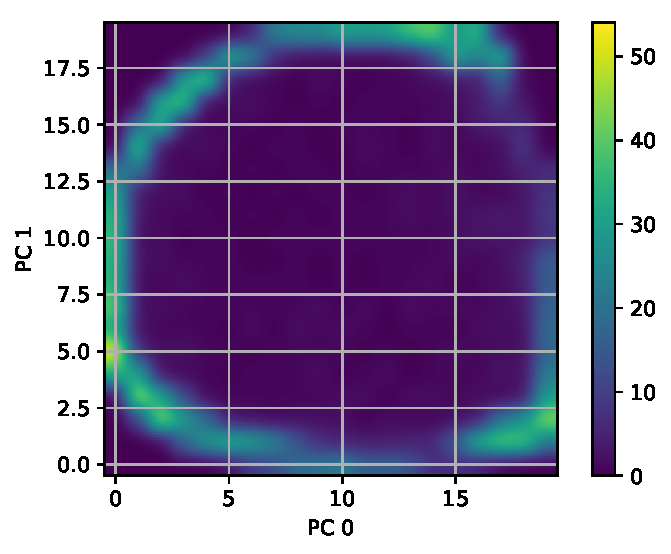
\includegraphics[]{figures/GeneratedSnapshots.pdf}
  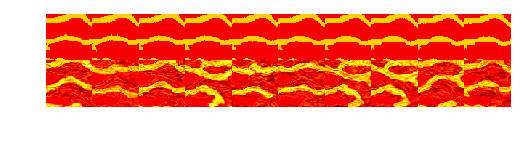
\includegraphics[]{figures/GeneratedSnapshots_KDESamples100.png}
  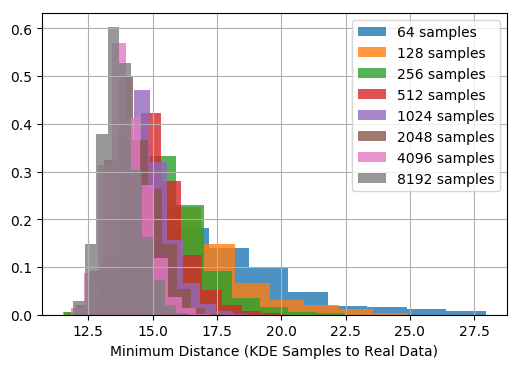
\includegraphics[]{figures/GeneratedSnapshots_KDESamplesPWD100.png}
  \caption{Plot of results for the application of PCA to $2500$ generated samples corresponding to a fixed category, fixed random noise sample, varying a single continuous latent variaable. Displayed are the Principal Modes (top), Joint Density of first two principal modes (upper middle), Realizations resulting from Kernel Density Estimation of the principal component basis.  Distribution of errors in KDE-sampled generations for increasing sample size.}
\end{figure}\label{GenPCA2}




\section{Conclusion}
	In conclusion, we find that all among training, validation, and test data can be partitioned across the categories determined by the GAN.  When partitioned according to the natural structure of the data, the generator is able to not only to combine like elements of a high-dimensional dataset, but also learns to construct the effect of qualitatively smooth transformations.  With this, a linear, closed-form mapping from a given snapshot to a continuous transformation thereof is feasible, allowing for optimization with respect to a smooth manifold.\label{GenPCA2} 

\subsubsection*{Acknowledgments And Notes}

As the author had no prior knowledge of Tensorflow, we note our appreciation for the highly insightful tutorials of Taehoon Kim, Arthur Juliani, and Ray Tsang.  As the content of the course was exceptionally interesting, we thank the reader for allowing us to enroll at a later time. Furthermore, we apologize for the delay with which this was sent, it was previously unreadable.





\bibliographystyle{unsrt}

\bibliography{Mendeley}

\end{document}
